\chapter{Systemkrav}\label{Systemkrav}
\section{Systembeskrivelse}
Automatisk Ultralydsscanner er et system, som gør det muligt at lave en automatiseret ultralydscanning af brystet mhp. screening for brystkræft. Systemet Automatisk Ultralydsscanner består af Robotarm, PC Applikation med en grafisk brugergrænseflade (GUI), 3D kamera og Ultralydsscanner. Se figur \ref{System} nedenfor. 

Via GUI kan en operatør, med kendskab til ultralyd, interagere med en PC applikation. Operatøren vælger først at udføre en 3D-scanning af patientets bryst. Derefter kan PC applikationen, ud fra 3D scanningen, udregne de positioner og rotationer der er nødvendige for at udføre en ultralydsscanning. For at kunne ultralydsscanne er det nødvendigt at påføre ultralydsgel. Dernæst vil operatøren vælge at påbegynde ultralydsscanningen, hvor en robotarm med påmonteret ultralydsprobe føres rundt på det detekterede brystområde på patienten. Ultralydsscanningsvideoen kan herefter sendes til undersøgelse.

Figur \ref{System} nedenfor viser en oversigt over, hvordan elementerne i Automatisk Ultralydsscanner interagerer med hinanden.
 
\begin{figure}[H]
    \centering
    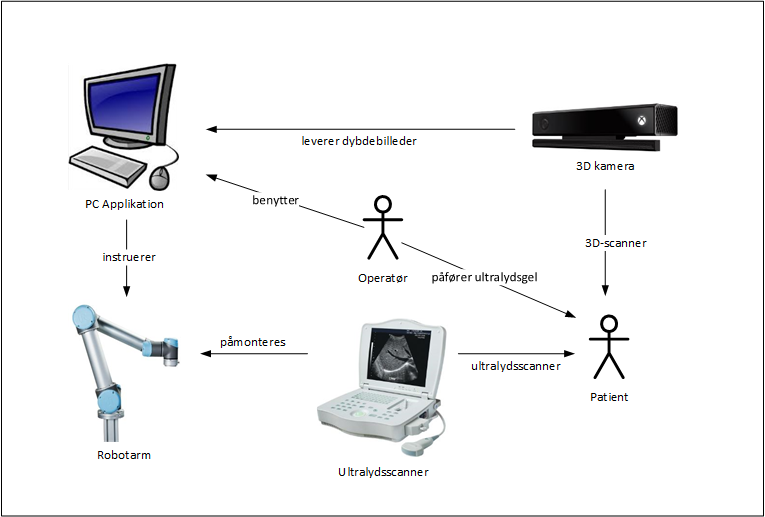
\includegraphics[width=0.75\textwidth]{figurer/d/Kravspecifikation/Systembeskrivelse}
    \caption{Systemoversigt over Automatisk Ultralydsscanner, der beskriver systemets opbygning og hvorledes de enkelte elementer interagerer}
    \label{System}
\end{figure}

\section{Aktører}
Der er identificeret fem aktører, som interagerer med systemet. Aktørerne inkluderer en operatør, en patient, en robotarm, en ultralydsscanner og et 3D kamera. PC Applikation ses som værende én samlet blok af PC og software, hvor softwaren er på PC. Operatør betjener PC Applikation, mens scanningen foregår på Patient. 3D kamera leverer dybdebilleder til PC Applikation. Robotarm styrer en påmonteret Ultralydsscanner i et specifikt overlappende bevægelsesmønster på det detekterede område.

\section{Funktionelle krav}
De funktionelle krav for Automatisk Ultralydsscanner er defineret ved brug af use cases (UC). Til systemet er der identificeret fire use cases, som kan ses i use case diagrammet på figur \ref{UseCaseDiagram} og i kravspecifikation, bilag \ref{Kravspecifikation}. 

Operatør gør klar til at 3D scanning ved at opstarte PC Applikation (UC1: Start System). Hovedmenuen på GUI vil vises, hvorpå Operatør kan vælge at 3D scanne Patients brystområde (UC2: 3D scan brystområde). Inden der kan ultralydsscannes, skal Operatør påføre en gel for at muliggøre ultralydsscanning. Operatøren har mulighed for at vælge at lave en ultralydsscanning ved tryk på en knap på GUI, hvorefter Robotarm vil køre over brystet (UC3: Ultrascan brystområde).  Operatør kan derefter på GUI vælge at stoppe systemet (UC4: Stop System). I figur \ref{UseCaseDiagram} nedenfor, vises Automatisk Ultralydsscanners Use Cases og aktørernes relation hertil.

\begin{figure}[H]
    \centering
    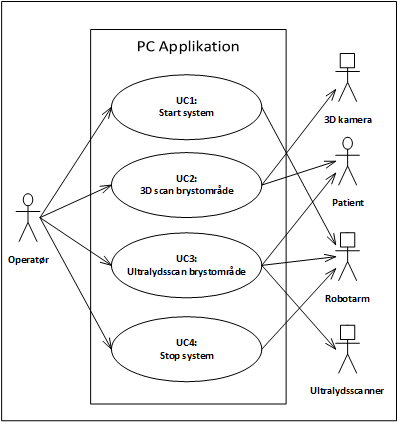
\includegraphics[width=0.75\textwidth]{figurer/d/Kravspecifikation/UseCaseDiagram}
    \caption{Use Case diagram for Automatisk Ultralydsscanner.}
    \label{UseCaseDiagram}
\end{figure}

\section{Ikke-funktionelle krav}
De ikke-funktionelle krav for Automatisk Ultralydsscanner er beskrevet ved brug af MoSCoW og FURPS+. Det er kun must-krav, der er implementeret og specielt performancestider for Automatisk Ultralydsscanners er prioriteret, for at systemet kan udføre en scanning på samme tid som en radiolog. Nedenfor kan de implementerede ikke-funktionelle krav ses. Se bilag \ref{Kravspecifikation} Kravspecifikation for at se krav, der ikke er blevet implementeret. 
I projektet er systemets performancetider blevet prioriteret højt, da det potentielt vil kunne forbedre mulighederne for implementering af Automatisk Ultralydsscanner i sundhedsvæsenet, hvor tid er en vigtig ressource. Derudover er det prioriteret, at Operatør nemt skal kunne anvende systemet, og derfor er der krav til en intuitiv GUI med feedback.

\subsubsection{Usability}
\begin{itemize}
    \item[U1.] PC Applikation skal have en GUI. (must)
    \item[U2.] GUI skal have en procent-indikator for ultralydsscanningens gennemløb. (must)
	\item[U3.] GUI skal vise en 3D model af 3D scanningen
\end{itemize}

\subsubsection{Performance}
\begin{itemize}
    \item[P1.] Scaningen med 3D kamera og ultralydsscanning skal max tage 10 minutter til sammen. (must) 
    \item[P2.] Starttid på PC Applikation skal være max 10 sekunder. (must)
    \item[P3.] 3D kamera skal max bruge 10 sekunder på at tage 3D billedet. (must)
    \item[P4.] PC Applikation skal max 10 sekunder på at færdiggøre brystområdets positurer til Robotarm. (must)
\end{itemize}

\subsection{Ekstra}
Lovkravene til medicinsk udstyr og medicinsk software, burde have været et must-krav i de ikke-funktionelle krav til Automatisk Ultralydsscanner, men da den medicinske godkendelse først blev udarbejdet sent i udviklingsprocessen er kravene fra den medicinske godkendelse ikke implementeret i systemet. Dette er for eksempel krav som at Automatisk Ultralydsscanner skal: 

\begin{itemize}
\item Designes så det ikke er til fare for Operatør og Patient. 
\item Fremstilles i et materiale som mindsker spredning af bakterier. 
\item Have tydelige og letforståelige tegn på knapper og display.
\item Have et risikohåndteringssystem \cite{13485}.
\item Have et kvalitetssikringssystem \cite{14971}. 
\item Mærkes så der ikke kan være tvivl om hvordan produktet skal bruges.
\item Kunne modstå en luftbåren ESD-transient på op til ±8 kiloVolt \cite{60601}.
\item Kunne tåle en indstråling på 3V/m \cite{60601}.
\end{itemize}

Punkter der ikke er markeret med referencer, stammer alle fra Medical Device Directive 93/42/EØF \cite{MDD}. 